%!TeX spellcheck = en_UK
% Die erste (unkommentierte) Zeile im Dokument legt immer die
% Dokumentklasse fest
\documentclass{scrartcl} 

% Präambel:
% Einbinen von zusätzlichen Paketen. Falls für eine Datei keine Endung
% explizit angegeben wird, benutzt LaTeX '.tex'. Im Folgenden wird
% also die Datei 'edv_pakete.tex' eingebunden.
% Die erste Zeile im Dokument legt immer die Dokumentklasse fest
%\documentclass[notitlepage]{scrreprt}
    % Die wichtigsten Dokumentklassen:
    %   scrbook, scrreprt, scrartcl, beamer, standalone
    % Einige gängige Optionen für \documentclass:
    %   ngerman
    %   titlepage, notitlepage
    %   onecolumn, twocolumn
    %   oneside, twoside
    %wird in Hauptdatei festgelegt

% Präambel

% Einige KOMA-Script-Optionen
\KOMAoptions{fontsize=12pt,paper=a4}      %Schriftgröße, Papierformat
\KOMAoptions{DIV=11}                      % Parameter mit dem man den Seitenrand ändern kann
\KOMAoptions{listof=totoc}

% Hier werden einige Pakete eingebunden
\usepackage[utf8]{inputenc}               % Direkte Eingabe von ä usw. Input=Eingabe
\usepackage[T1]{fontenc}                  % Font Kodierung für die Ausgabe Font=Ausgabe
\usepackage[english]{babel}               % Verschiedenste sprach-spezifische Extras, ngerman für neue deutsche Rechtschreibung, auch UK oder US möglich
\usepackage[autostyle=true]{csquotes}     % Intelligente Anführungszeichen, arbeitet mit Babel zusammen
%

\usepackage{amsmath}%Mathedarstellung
\usepackage{commath}%Mathedarstellung
\usepackage{physics}%Physik-Symbole
%\usepackage{IEEEtrantools}%IEEEeqnarray
%
\usepackage{siunitx}   % Intelligentes Setzen von Zahlen und Einheiten
%\sisetup{locale = DE}  % Deutsch als locale für die Zahlen und Einheiten
%http://tex.stackexchange.com/questions/2291/how-do-i-change-the-enumerate-list-format-to-use-letters-instead-of-the-defaul

\usepackage{enumitem}%erlaubt u.A. die Aufzählung mit Buchstaben, gefunden auf http://tex.stackexchange.com/questions/2291/how-do-i-change-the-enumerate-list-format-to-use-letters-instead-of-the-defaul
%
\usepackage[varg]{txfonts}                % Schönere Schriftart, muss nach amsmath, damit keine Fehlermeldung kommt
\usepackage{graphicx} %einbinden von Figuren/Bildern
\graphicspath{{figs/}} % Stammverzeichnis der verwendeten Bilder, muss im selben Ordner wie Hauptdatei sein
%
\usepackage[backend=biber, style=numeric, sorting=none]{biblatex}
%Verwenden von \cite in \footnote: Bibliographie drucken lassen, mehrmals kompilieren
\usepackage{hyperref}%erzeugt klickbare Elemente
\usepackage[all]{hypcap}%hyperref-befehle springen zum oberen Rand des Bildes
% Zum Einbinden von Programmcode verwenden wir das listings-Paket
\usepackage{listings}

% Für Syntax-Highlighting:
\usepackage{xcolor}

\usepackage{longtable}

% Die folgenden listings-Einstellungen sind nötig, um
% deutsche Umlaute und die Tilde (~) in listings-Umgebungen
% verwenden zu können.
\lstset{
    basicstyle=\ttfamily,    
    literate={~} {$\sim$}{1} % set tilde as a literal
    {ö}{{\"o}}1
    {ä}{{\"a}}1
    {ü}{{\"u}}1
    {ß}{{\ss}}1
    {Ö}{{\"O}}1
    {Ä}{{\"A}}1
    {Ü}{{\"U}}1
}

% Farben für Code-Syntaxhighlighting und Weiteres festlegen:
\lstset{
    % Keine besondere Markierung für Leerzeichen in Codes
    showspaces=false,               
    showstringspaces=false,         
    % Farebn für Code-Kommentare und Schlüsselworte:
    commentstyle=\color{red},       % comment style
    keywordstyle=\color{blue},      % keyword style
    stringstyle=\color{orange},		% string style
    breaklines=true,
    numbers=left,                    % where to put the line-numbers; possible values are (none, left, right)
    numbersep=5pt,                   % how far the line-numbers are from the code
    stepnumber=5, 					%how often there are line numbers in code listings
    tabsize=4, 						%default tabsize set to 4 spaces
    %language=python,
    }
%gefunden auf https://en.wikibooks.org/wiki/LaTeX/Source_Code_Listings
%eigene Kommandos/Abürzungen
\newcommand{\tb}{\textbackslash}
\newcommand{\txt}{\texttt}
\newcommand{\umt}{u_{(i+i\%2)/2}^{(2a)}}
\newcommand{\utmt}{u_{(i-2+i\%2)/2}^{(2a)}}
\newcommand{\uti}{\tilde{u}_i^{(a)}}
\newcommand{\utio}{\tilde{u}_{i-1}^{(a)}}




% Verzeichnisse mit Abbildungen; kann gestrichen werden,
% falls Sie dies schon in edv_pakete.tex definiert haben:
%\graphicspath{{../report}}

\addbibresource{refs.bib} %Hinzufügen einer Literaturdatenbank aus dem angegebenen Verzeichnis

% Titel, Autor und Datum
\title{Computational Physics}
\subtitle{Exercise 4}
\date{\today}
\author{Christiane Groß, Nico Dichter}

% Jetzt startet das eigentliche Dokument
\begin{document}
	\maketitle
\section{Error Analysis of a Markov Chain}
All of our calculations are based on definitions and principles introduced in the lectures or on the exercise sheets.
\subsection{Simulated Model}
We want to analyse the Markov-chains produced when looking at the magnetization of long-range Ising-model simulated with the Hybrid Monte Carlo algorithm. We already implemented this algorithm in exercise 3, and it describes N spins that all interact with each other and with the external magnetic field. For the analysis of the errors, we only look at the internal coupling $\beta J=0.1$ and the external magnetic field $\beta h=0.5$ for $N=5$ spins. 
 
In the HMC algorithm, we evolve a given $\phi$ and a $p$ sampled from a normal distribution according to their equations of motion with the help of a molecular dynamics integrator, in our case a leapfrog integrator, to $\phi', p'$ and accepting these new values with a probability of $\min(1, \exp(H(\phi, p)-H(\phi', p')))$. Here we look at the differences that occur when using a different number of steps in the leapfrog algorithm, specifically $N_{md}=4$ and $N_{md}=100$.

From these $\phi$ we can then calculate the magnetization $m=\tanh(\beta h+\phi)$.

\subsection{Autocorrelation}

Because we produce the magnetization with the value of $\phi$ from the last measurement, we know these measurements are autocorrelated. We measure this correlation by calculating the autocorrelation function as given in the lecture:
\[
C(\tau)=\frac{1}{N-|\tau|}\sum_{i=1}^{N-|\tau|}(O_i-\bar{\mu})(O_{i+|\tau|}-\bar{\mu})\]

Here $N$ is the number of measurements, the $O_i$ are a single measurement, and $\bar{\mu}$ is the estimated mean. To make visualotsation and comparison easier, we look at the normalised autocorrelation function, \[
\Gamma(\tau)=\frac{C(\tau)}{C(0)}
\]

\subsection{Binning}

Trying to reduce the autocorrelation, we do not look at single measurements any more, but instead we form blocks, also called bins, of the measurements. For $N$ measurements, we cann form $\lfloor N/l \rfloor$ blocks of length $l$, where the k-th block is defined as \[O_k^B=\frac{1}{l}\sum_{i=0}^{l-1}O_{(k\cdot l)+i}\].

\subsection{Bootstrapping}

%From these new datapoints, we make $R$ bootstrap replicas. For each replica, we sample with replacement from the given $O_i^B$, and take the arithmetic mean over those chosen values to be the replica. At the end, we can estimate the mean and error of our measurements as the arithmetic mean and standard deviation over $R$ bootstrap replicas.

For a realistic error estimate, we would need to perform several sets of measurements and compare their means. Because this is not possible, we simulate $R$ sets of measurements by making so called bootstrap replicas: For one replica, we randomly sample with replacement from our measurements. If we have $N$ measurements $x_i$, we draw $N$ samples $x_i^s$. The arithmetic mean of these samples, $\mu^s_j=\frac{1}{N}\sum_{i=0}^{N-1}x_i^s$, is one replica.

From our replica, we calculate the mean $\bar{\mu}$ and the error $\bar{\sigma}$ of our measurements as the simple arithmetic mean and the simple standard deviation of the replica.
\[
\bar{\mu}=\frac{1}{R}\sum_{j=0}^{R-1}\mu^s_j\]


\[
\bar{\sigma}^2=\frac{1}{R-1}\sum_{j=0}^{R-1}(\mu^s_j-\bar{\mu})^2
\]

\section{Implementation}
Our code is in the github-repo \url{https://github.com/christianegross/CompPhys\_2021}. The simulation itself is in Exercise4/src/main/main.c, the gnuplotscript, where we have also implemented the expectations for the magnetization and energy is in Exercise4/report/plot.gp.

\section{Results}

\subsection{Comparison of Markov Chains with different $N_{md}$}

\begin{figure}[htbp]
	% GNUPLOT: LaTeX picture with Postscript
\begingroup
  \makeatletter
  \providecommand\color[2][]{%
    \GenericError{(gnuplot) \space\space\space\@spaces}{%
      Package color not loaded in conjunction with
      terminal option `colourtext'%
    }{See the gnuplot documentation for explanation.%
    }{Either use 'blacktext' in gnuplot or load the package
      color.sty in LaTeX.}%
    \renewcommand\color[2][]{}%
  }%
  \providecommand\includegraphics[2][]{%
    \GenericError{(gnuplot) \space\space\space\@spaces}{%
      Package graphicx or graphics not loaded%
    }{See the gnuplot documentation for explanation.%
    }{The gnuplot epslatex terminal needs graphicx.sty or graphics.sty.}%
    \renewcommand\includegraphics[2][]{}%
  }%
  \providecommand\rotatebox[2]{#2}%
  \@ifundefined{ifGPcolor}{%
    \newif\ifGPcolor
    \GPcolortrue
  }{}%
  \@ifundefined{ifGPblacktext}{%
    \newif\ifGPblacktext
    \GPblacktextfalse
  }{}%
  % define a \g@addto@macro without @ in the name:
  \let\gplgaddtomacro\g@addto@macro
  % define empty templates for all commands taking text:
  \gdef\gplbacktext{}%
  \gdef\gplfronttext{}%
  \makeatother
  \ifGPblacktext
    % no textcolor at all
    \def\colorrgb#1{}%
    \def\colorgray#1{}%
  \else
    % gray or color?
    \ifGPcolor
      \def\colorrgb#1{\color[rgb]{#1}}%
      \def\colorgray#1{\color[gray]{#1}}%
      \expandafter\def\csname LTw\endcsname{\color{white}}%
      \expandafter\def\csname LTb\endcsname{\color{black}}%
      \expandafter\def\csname LTa\endcsname{\color{black}}%
      \expandafter\def\csname LT0\endcsname{\color[rgb]{1,0,0}}%
      \expandafter\def\csname LT1\endcsname{\color[rgb]{0,1,0}}%
      \expandafter\def\csname LT2\endcsname{\color[rgb]{0,0,1}}%
      \expandafter\def\csname LT3\endcsname{\color[rgb]{1,0,1}}%
      \expandafter\def\csname LT4\endcsname{\color[rgb]{0,1,1}}%
      \expandafter\def\csname LT5\endcsname{\color[rgb]{1,1,0}}%
      \expandafter\def\csname LT6\endcsname{\color[rgb]{0,0,0}}%
      \expandafter\def\csname LT7\endcsname{\color[rgb]{1,0.3,0}}%
      \expandafter\def\csname LT8\endcsname{\color[rgb]{0.5,0.5,0.5}}%
    \else
      % gray
      \def\colorrgb#1{\color{black}}%
      \def\colorgray#1{\color[gray]{#1}}%
      \expandafter\def\csname LTw\endcsname{\color{white}}%
      \expandafter\def\csname LTb\endcsname{\color{black}}%
      \expandafter\def\csname LTa\endcsname{\color{black}}%
      \expandafter\def\csname LT0\endcsname{\color{black}}%
      \expandafter\def\csname LT1\endcsname{\color{black}}%
      \expandafter\def\csname LT2\endcsname{\color{black}}%
      \expandafter\def\csname LT3\endcsname{\color{black}}%
      \expandafter\def\csname LT4\endcsname{\color{black}}%
      \expandafter\def\csname LT5\endcsname{\color{black}}%
      \expandafter\def\csname LT6\endcsname{\color{black}}%
      \expandafter\def\csname LT7\endcsname{\color{black}}%
      \expandafter\def\csname LT8\endcsname{\color{black}}%
    \fi
  \fi
    \setlength{\unitlength}{0.0500bp}%
    \ifx\gptboxheight\undefined%
      \newlength{\gptboxheight}%
      \newlength{\gptboxwidth}%
      \newsavebox{\gptboxtext}%
    \fi%
    \setlength{\fboxrule}{0.5pt}%
    \setlength{\fboxsep}{1pt}%
\begin{picture}(8502.00,5668.00)%
    \gplgaddtomacro\gplbacktext{%
      \csname LTb\endcsname%
      \put(814,704){\makebox(0,0)[r]{\strut{}$0$}}%
      \put(814,1291){\makebox(0,0)[r]{\strut{}$0.1$}}%
      \put(814,1879){\makebox(0,0)[r]{\strut{}$0.2$}}%
      \put(814,2466){\makebox(0,0)[r]{\strut{}$0.3$}}%
      \put(814,3054){\makebox(0,0)[r]{\strut{}$0.4$}}%
      \put(814,3641){\makebox(0,0)[r]{\strut{}$0.5$}}%
      \put(814,4228){\makebox(0,0)[r]{\strut{}$0.6$}}%
      \put(814,4816){\makebox(0,0)[r]{\strut{}$0.7$}}%
      \put(814,5403){\makebox(0,0)[r]{\strut{}$0.8$}}%
      \put(946,484){\makebox(0,0){\strut{}$0$}}%
      \put(2378,484){\makebox(0,0){\strut{}$100$}}%
      \put(3810,484){\makebox(0,0){\strut{}$200$}}%
      \put(5241,484){\makebox(0,0){\strut{}$300$}}%
      \put(6673,484){\makebox(0,0){\strut{}$400$}}%
      \put(8105,484){\makebox(0,0){\strut{}$500$}}%
    }%
    \gplgaddtomacro\gplfronttext{%
      \csname LTb\endcsname%
      \put(176,3053){\rotatebox{-270}{\makebox(0,0){\strut{}magnetization}}}%
      \put(4525,154){\makebox(0,0){\strut{}time}}%
      \csname LTb\endcsname%
      \put(7118,5230){\makebox(0,0)[r]{\strut{}$N_{md}=4$}}%
      \csname LTb\endcsname%
      \put(7118,5010){\makebox(0,0)[r]{\strut{}$N_{md}=100$}}%
    }%
    \gplbacktext
    \put(0,0){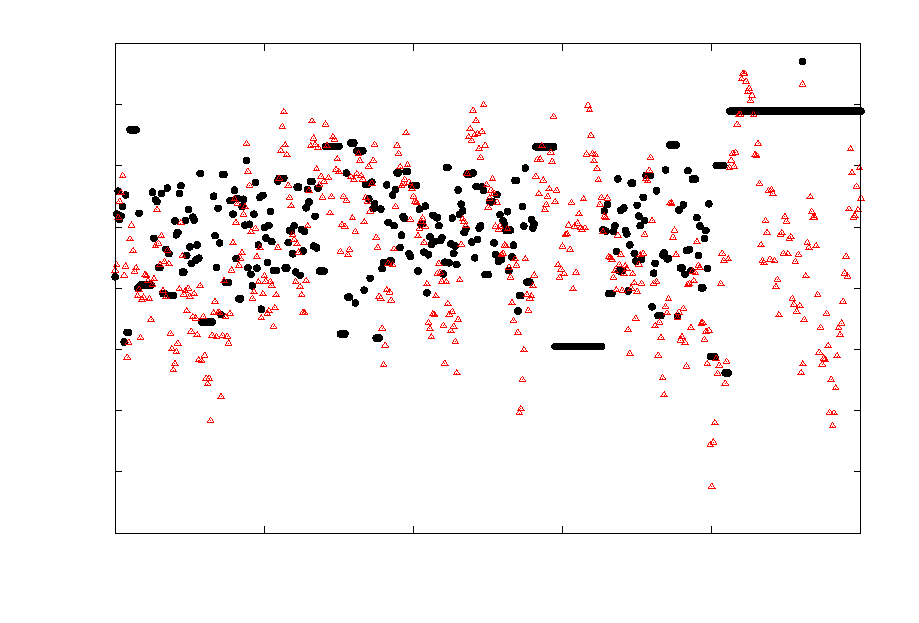
\includegraphics{markovchaincomparison}}%
    \gplfronttext
  \end{picture}%
\endgroup

	\caption{Comparison of two Markov Chains with the same parameters except for $N_{md}=4, 100$}
	\label{fig:markovchaincomparison}
\end{figure}



\subsection{Autocorrelation of the measurements}


\begin{figure}[htbp]
	% GNUPLOT: LaTeX picture with Postscript
\begingroup
  \makeatletter
  \providecommand\color[2][]{%
    \GenericError{(gnuplot) \space\space\space\@spaces}{%
      Package color not loaded in conjunction with
      terminal option `colourtext'%
    }{See the gnuplot documentation for explanation.%
    }{Either use 'blacktext' in gnuplot or load the package
      color.sty in LaTeX.}%
    \renewcommand\color[2][]{}%
  }%
  \providecommand\includegraphics[2][]{%
    \GenericError{(gnuplot) \space\space\space\@spaces}{%
      Package graphicx or graphics not loaded%
    }{See the gnuplot documentation for explanation.%
    }{The gnuplot epslatex terminal needs graphicx.sty or graphics.sty.}%
    \renewcommand\includegraphics[2][]{}%
  }%
  \providecommand\rotatebox[2]{#2}%
  \@ifundefined{ifGPcolor}{%
    \newif\ifGPcolor
    \GPcolortrue
  }{}%
  \@ifundefined{ifGPblacktext}{%
    \newif\ifGPblacktext
    \GPblacktextfalse
  }{}%
  % define a \g@addto@macro without @ in the name:
  \let\gplgaddtomacro\g@addto@macro
  % define empty templates for all commands taking text:
  \gdef\gplbacktext{}%
  \gdef\gplfronttext{}%
  \makeatother
  \ifGPblacktext
    % no textcolor at all
    \def\colorrgb#1{}%
    \def\colorgray#1{}%
  \else
    % gray or color?
    \ifGPcolor
      \def\colorrgb#1{\color[rgb]{#1}}%
      \def\colorgray#1{\color[gray]{#1}}%
      \expandafter\def\csname LTw\endcsname{\color{white}}%
      \expandafter\def\csname LTb\endcsname{\color{black}}%
      \expandafter\def\csname LTa\endcsname{\color{black}}%
      \expandafter\def\csname LT0\endcsname{\color[rgb]{1,0,0}}%
      \expandafter\def\csname LT1\endcsname{\color[rgb]{0,1,0}}%
      \expandafter\def\csname LT2\endcsname{\color[rgb]{0,0,1}}%
      \expandafter\def\csname LT3\endcsname{\color[rgb]{1,0,1}}%
      \expandafter\def\csname LT4\endcsname{\color[rgb]{0,1,1}}%
      \expandafter\def\csname LT5\endcsname{\color[rgb]{1,1,0}}%
      \expandafter\def\csname LT6\endcsname{\color[rgb]{0,0,0}}%
      \expandafter\def\csname LT7\endcsname{\color[rgb]{1,0.3,0}}%
      \expandafter\def\csname LT8\endcsname{\color[rgb]{0.5,0.5,0.5}}%
    \else
      % gray
      \def\colorrgb#1{\color{black}}%
      \def\colorgray#1{\color[gray]{#1}}%
      \expandafter\def\csname LTw\endcsname{\color{white}}%
      \expandafter\def\csname LTb\endcsname{\color{black}}%
      \expandafter\def\csname LTa\endcsname{\color{black}}%
      \expandafter\def\csname LT0\endcsname{\color{black}}%
      \expandafter\def\csname LT1\endcsname{\color{black}}%
      \expandafter\def\csname LT2\endcsname{\color{black}}%
      \expandafter\def\csname LT3\endcsname{\color{black}}%
      \expandafter\def\csname LT4\endcsname{\color{black}}%
      \expandafter\def\csname LT5\endcsname{\color{black}}%
      \expandafter\def\csname LT6\endcsname{\color{black}}%
      \expandafter\def\csname LT7\endcsname{\color{black}}%
      \expandafter\def\csname LT8\endcsname{\color{black}}%
    \fi
  \fi
    \setlength{\unitlength}{0.0500bp}%
    \ifx\gptboxheight\undefined%
      \newlength{\gptboxheight}%
      \newlength{\gptboxwidth}%
      \newsavebox{\gptboxtext}%
    \fi%
    \setlength{\fboxrule}{0.5pt}%
    \setlength{\fboxsep}{1pt}%
\begin{picture}(8502.00,5668.00)%
    \gplgaddtomacro\gplbacktext{%
      \csname LTb\endcsname%
      \put(946,704){\makebox(0,0)[r]{\strut{}$-0.2$}}%
      \put(946,1487){\makebox(0,0)[r]{\strut{}$0$}}%
      \put(946,2270){\makebox(0,0)[r]{\strut{}$0.2$}}%
      \put(946,3054){\makebox(0,0)[r]{\strut{}$0.4$}}%
      \put(946,3837){\makebox(0,0)[r]{\strut{}$0.6$}}%
      \put(946,4620){\makebox(0,0)[r]{\strut{}$0.8$}}%
      \put(946,5403){\makebox(0,0)[r]{\strut{}$1$}}%
      \put(1078,484){\makebox(0,0){\strut{}$0$}}%
      \put(2483,484){\makebox(0,0){\strut{}$100$}}%
      \put(3889,484){\makebox(0,0){\strut{}$200$}}%
      \put(5294,484){\makebox(0,0){\strut{}$300$}}%
      \put(6700,484){\makebox(0,0){\strut{}$400$}}%
      \put(8105,484){\makebox(0,0){\strut{}$500$}}%
    }%
    \gplgaddtomacro\gplfronttext{%
      \csname LTb\endcsname%
      \put(176,3053){\rotatebox{-270}{\makebox(0,0){\strut{}$\Gamma(\tau)$}}}%
      \put(4591,154){\makebox(0,0){\strut{}time}}%
      \csname LTb\endcsname%
      \put(7118,5230){\makebox(0,0)[r]{\strut{}$N_{md}=4$}}%
      \csname LTb\endcsname%
      \put(7118,5010){\makebox(0,0)[r]{\strut{}$N_{md}=100$}}%
    }%
    \gplbacktext
    \put(0,0){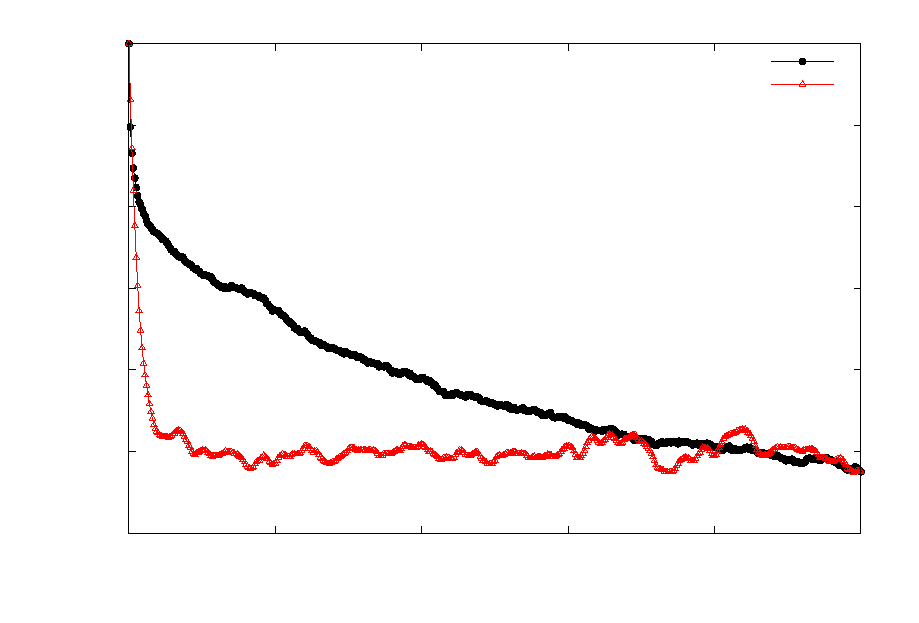
\includegraphics{simplecorrelation}}%
    \gplfronttext
  \end{picture}%
\endgroup

	\caption{Autocorrelation of the Markov Chains from fig.~\ref{fig:markovchaincomparison}.}
	\label{fig:simplecorrelation}
\end{figure}

\begin{figure}[htbp]
	% GNUPLOT: LaTeX picture with Postscript
\begingroup
  \makeatletter
  \providecommand\color[2][]{%
    \GenericError{(gnuplot) \space\space\space\@spaces}{%
      Package color not loaded in conjunction with
      terminal option `colourtext'%
    }{See the gnuplot documentation for explanation.%
    }{Either use 'blacktext' in gnuplot or load the package
      color.sty in LaTeX.}%
    \renewcommand\color[2][]{}%
  }%
  \providecommand\includegraphics[2][]{%
    \GenericError{(gnuplot) \space\space\space\@spaces}{%
      Package graphicx or graphics not loaded%
    }{See the gnuplot documentation for explanation.%
    }{The gnuplot epslatex terminal needs graphicx.sty or graphics.sty.}%
    \renewcommand\includegraphics[2][]{}%
  }%
  \providecommand\rotatebox[2]{#2}%
  \@ifundefined{ifGPcolor}{%
    \newif\ifGPcolor
    \GPcolortrue
  }{}%
  \@ifundefined{ifGPblacktext}{%
    \newif\ifGPblacktext
    \GPblacktextfalse
  }{}%
  % define a \g@addto@macro without @ in the name:
  \let\gplgaddtomacro\g@addto@macro
  % define empty templates for all commands taking text:
  \gdef\gplbacktext{}%
  \gdef\gplfronttext{}%
  \makeatother
  \ifGPblacktext
    % no textcolor at all
    \def\colorrgb#1{}%
    \def\colorgray#1{}%
  \else
    % gray or color?
    \ifGPcolor
      \def\colorrgb#1{\color[rgb]{#1}}%
      \def\colorgray#1{\color[gray]{#1}}%
      \expandafter\def\csname LTw\endcsname{\color{white}}%
      \expandafter\def\csname LTb\endcsname{\color{black}}%
      \expandafter\def\csname LTa\endcsname{\color{black}}%
      \expandafter\def\csname LT0\endcsname{\color[rgb]{1,0,0}}%
      \expandafter\def\csname LT1\endcsname{\color[rgb]{0,1,0}}%
      \expandafter\def\csname LT2\endcsname{\color[rgb]{0,0,1}}%
      \expandafter\def\csname LT3\endcsname{\color[rgb]{1,0,1}}%
      \expandafter\def\csname LT4\endcsname{\color[rgb]{0,1,1}}%
      \expandafter\def\csname LT5\endcsname{\color[rgb]{1,1,0}}%
      \expandafter\def\csname LT6\endcsname{\color[rgb]{0,0,0}}%
      \expandafter\def\csname LT7\endcsname{\color[rgb]{1,0.3,0}}%
      \expandafter\def\csname LT8\endcsname{\color[rgb]{0.5,0.5,0.5}}%
    \else
      % gray
      \def\colorrgb#1{\color{black}}%
      \def\colorgray#1{\color[gray]{#1}}%
      \expandafter\def\csname LTw\endcsname{\color{white}}%
      \expandafter\def\csname LTb\endcsname{\color{black}}%
      \expandafter\def\csname LTa\endcsname{\color{black}}%
      \expandafter\def\csname LT0\endcsname{\color{black}}%
      \expandafter\def\csname LT1\endcsname{\color{black}}%
      \expandafter\def\csname LT2\endcsname{\color{black}}%
      \expandafter\def\csname LT3\endcsname{\color{black}}%
      \expandafter\def\csname LT4\endcsname{\color{black}}%
      \expandafter\def\csname LT5\endcsname{\color{black}}%
      \expandafter\def\csname LT6\endcsname{\color{black}}%
      \expandafter\def\csname LT7\endcsname{\color{black}}%
      \expandafter\def\csname LT8\endcsname{\color{black}}%
    \fi
  \fi
    \setlength{\unitlength}{0.0500bp}%
    \ifx\gptboxheight\undefined%
      \newlength{\gptboxheight}%
      \newlength{\gptboxwidth}%
      \newsavebox{\gptboxtext}%
    \fi%
    \setlength{\fboxrule}{0.5pt}%
    \setlength{\fboxsep}{1pt}%
\begin{picture}(8502.00,5668.00)%
    \gplgaddtomacro\gplbacktext{%
      \csname LTb\endcsname%
      \put(946,704){\makebox(0,0)[r]{\strut{}$-0.4$}}%
      \put(946,1375){\makebox(0,0)[r]{\strut{}$-0.2$}}%
      \put(946,2047){\makebox(0,0)[r]{\strut{}$0$}}%
      \put(946,2718){\makebox(0,0)[r]{\strut{}$0.2$}}%
      \put(946,3389){\makebox(0,0)[r]{\strut{}$0.4$}}%
      \put(946,4060){\makebox(0,0)[r]{\strut{}$0.6$}}%
      \put(946,4732){\makebox(0,0)[r]{\strut{}$0.8$}}%
      \put(946,5403){\makebox(0,0)[r]{\strut{}$1$}}%
      \put(1078,484){\makebox(0,0){\strut{}$0$}}%
      \put(2483,484){\makebox(0,0){\strut{}$20$}}%
      \put(3889,484){\makebox(0,0){\strut{}$40$}}%
      \put(5294,484){\makebox(0,0){\strut{}$60$}}%
      \put(6700,484){\makebox(0,0){\strut{}$80$}}%
      \put(8105,484){\makebox(0,0){\strut{}$100$}}%
    }%
    \gplgaddtomacro\gplfronttext{%
      \csname LTb\endcsname%
      \put(176,3053){\rotatebox{-270}{\makebox(0,0){\strut{}$\Gamma(\tau)$}}}%
      \put(4591,154){\makebox(0,0){\strut{}time}}%
      \csname LTb\endcsname%
      \put(7118,5230){\makebox(0,0)[r]{\strut{}binlength=2}}%
      \csname LTb\endcsname%
      \put(7118,5010){\makebox(0,0)[r]{\strut{}binlength=4}}%
      \csname LTb\endcsname%
      \put(7118,4790){\makebox(0,0)[r]{\strut{}binlength=8}}%
      \csname LTb\endcsname%
      \put(7118,4570){\makebox(0,0)[r]{\strut{}binlength=16}}%
      \csname LTb\endcsname%
      \put(7118,4350){\makebox(0,0)[r]{\strut{}binlength=32}}%
      \csname LTb\endcsname%
      \put(7118,4130){\makebox(0,0)[r]{\strut{}binlength=64}}%
    }%
    \gplbacktext
    \put(0,0){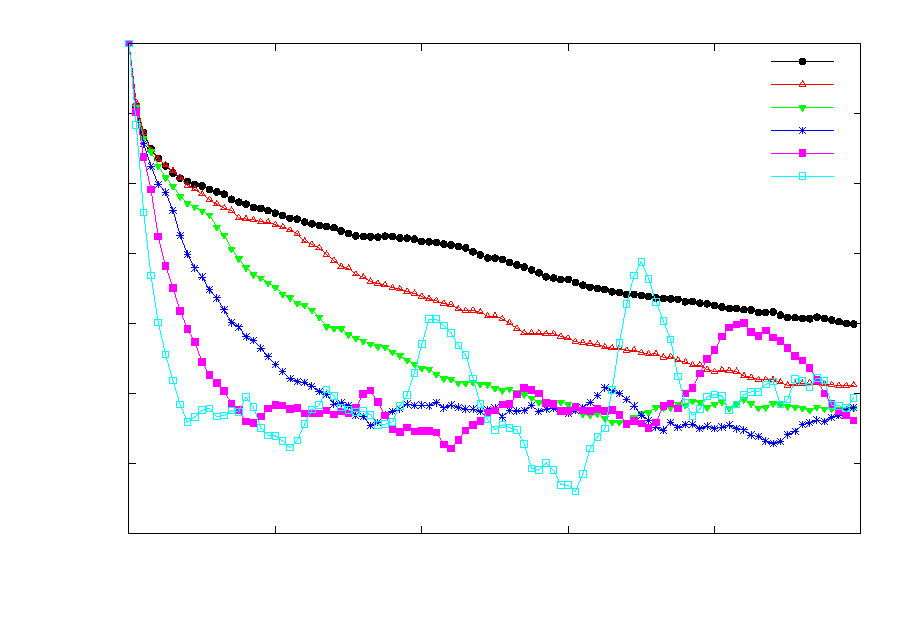
\includegraphics{correlationbinnmd4}}%
    \gplfronttext
  \end{picture}%
\endgroup

	\caption{Autocorrelation of the blocked Markov Chains for $N_{md}=4$}
	\label{fig:correlationbinnmd4}
\end{figure}

\begin{figure}[htbp]
	% GNUPLOT: LaTeX picture with Postscript
\begingroup
  \makeatletter
  \providecommand\color[2][]{%
    \GenericError{(gnuplot) \space\space\space\@spaces}{%
      Package color not loaded in conjunction with
      terminal option `colourtext'%
    }{See the gnuplot documentation for explanation.%
    }{Either use 'blacktext' in gnuplot or load the package
      color.sty in LaTeX.}%
    \renewcommand\color[2][]{}%
  }%
  \providecommand\includegraphics[2][]{%
    \GenericError{(gnuplot) \space\space\space\@spaces}{%
      Package graphicx or graphics not loaded%
    }{See the gnuplot documentation for explanation.%
    }{The gnuplot epslatex terminal needs graphicx.sty or graphics.sty.}%
    \renewcommand\includegraphics[2][]{}%
  }%
  \providecommand\rotatebox[2]{#2}%
  \@ifundefined{ifGPcolor}{%
    \newif\ifGPcolor
    \GPcolortrue
  }{}%
  \@ifundefined{ifGPblacktext}{%
    \newif\ifGPblacktext
    \GPblacktextfalse
  }{}%
  % define a \g@addto@macro without @ in the name:
  \let\gplgaddtomacro\g@addto@macro
  % define empty templates for all commands taking text:
  \gdef\gplbacktext{}%
  \gdef\gplfronttext{}%
  \makeatother
  \ifGPblacktext
    % no textcolor at all
    \def\colorrgb#1{}%
    \def\colorgray#1{}%
  \else
    % gray or color?
    \ifGPcolor
      \def\colorrgb#1{\color[rgb]{#1}}%
      \def\colorgray#1{\color[gray]{#1}}%
      \expandafter\def\csname LTw\endcsname{\color{white}}%
      \expandafter\def\csname LTb\endcsname{\color{black}}%
      \expandafter\def\csname LTa\endcsname{\color{black}}%
      \expandafter\def\csname LT0\endcsname{\color[rgb]{1,0,0}}%
      \expandafter\def\csname LT1\endcsname{\color[rgb]{0,1,0}}%
      \expandafter\def\csname LT2\endcsname{\color[rgb]{0,0,1}}%
      \expandafter\def\csname LT3\endcsname{\color[rgb]{1,0,1}}%
      \expandafter\def\csname LT4\endcsname{\color[rgb]{0,1,1}}%
      \expandafter\def\csname LT5\endcsname{\color[rgb]{1,1,0}}%
      \expandafter\def\csname LT6\endcsname{\color[rgb]{0,0,0}}%
      \expandafter\def\csname LT7\endcsname{\color[rgb]{1,0.3,0}}%
      \expandafter\def\csname LT8\endcsname{\color[rgb]{0.5,0.5,0.5}}%
    \else
      % gray
      \def\colorrgb#1{\color{black}}%
      \def\colorgray#1{\color[gray]{#1}}%
      \expandafter\def\csname LTw\endcsname{\color{white}}%
      \expandafter\def\csname LTb\endcsname{\color{black}}%
      \expandafter\def\csname LTa\endcsname{\color{black}}%
      \expandafter\def\csname LT0\endcsname{\color{black}}%
      \expandafter\def\csname LT1\endcsname{\color{black}}%
      \expandafter\def\csname LT2\endcsname{\color{black}}%
      \expandafter\def\csname LT3\endcsname{\color{black}}%
      \expandafter\def\csname LT4\endcsname{\color{black}}%
      \expandafter\def\csname LT5\endcsname{\color{black}}%
      \expandafter\def\csname LT6\endcsname{\color{black}}%
      \expandafter\def\csname LT7\endcsname{\color{black}}%
      \expandafter\def\csname LT8\endcsname{\color{black}}%
    \fi
  \fi
    \setlength{\unitlength}{0.0500bp}%
    \ifx\gptboxheight\undefined%
      \newlength{\gptboxheight}%
      \newlength{\gptboxwidth}%
      \newsavebox{\gptboxtext}%
    \fi%
    \setlength{\fboxrule}{0.5pt}%
    \setlength{\fboxsep}{1pt}%
\begin{picture}(8502.00,5668.00)%
    \gplgaddtomacro\gplbacktext{%
      \csname LTb\endcsname%
      \put(946,704){\makebox(0,0)[r]{\strut{}$-0.2$}}%
      \put(946,1487){\makebox(0,0)[r]{\strut{}$0$}}%
      \put(946,2270){\makebox(0,0)[r]{\strut{}$0.2$}}%
      \put(946,3054){\makebox(0,0)[r]{\strut{}$0.4$}}%
      \put(946,3837){\makebox(0,0)[r]{\strut{}$0.6$}}%
      \put(946,4620){\makebox(0,0)[r]{\strut{}$0.8$}}%
      \put(946,5403){\makebox(0,0)[r]{\strut{}$1$}}%
      \put(1078,484){\makebox(0,0){\strut{}$0$}}%
      \put(2483,484){\makebox(0,0){\strut{}$10$}}%
      \put(3889,484){\makebox(0,0){\strut{}$20$}}%
      \put(5294,484){\makebox(0,0){\strut{}$30$}}%
      \put(6700,484){\makebox(0,0){\strut{}$40$}}%
      \put(8105,484){\makebox(0,0){\strut{}$50$}}%
    }%
    \gplgaddtomacro\gplfronttext{%
      \csname LTb\endcsname%
      \put(176,3053){\rotatebox{-270}{\makebox(0,0){\strut{}$\Gamma(\tau)$}}}%
      \put(4591,154){\makebox(0,0){\strut{}time}}%
      \csname LTb\endcsname%
      \put(7118,5230){\makebox(0,0)[r]{\strut{}binlength=2}}%
      \csname LTb\endcsname%
      \put(7118,5010){\makebox(0,0)[r]{\strut{}binlength=4}}%
      \csname LTb\endcsname%
      \put(7118,4790){\makebox(0,0)[r]{\strut{}binlength=8}}%
      \csname LTb\endcsname%
      \put(7118,4570){\makebox(0,0)[r]{\strut{}binlength=16}}%
      \csname LTb\endcsname%
      \put(7118,4350){\makebox(0,0)[r]{\strut{}binlength=32}}%
      \csname LTb\endcsname%
      \put(7118,4130){\makebox(0,0)[r]{\strut{}binlength=64}}%
    }%
    \gplbacktext
    \put(0,0){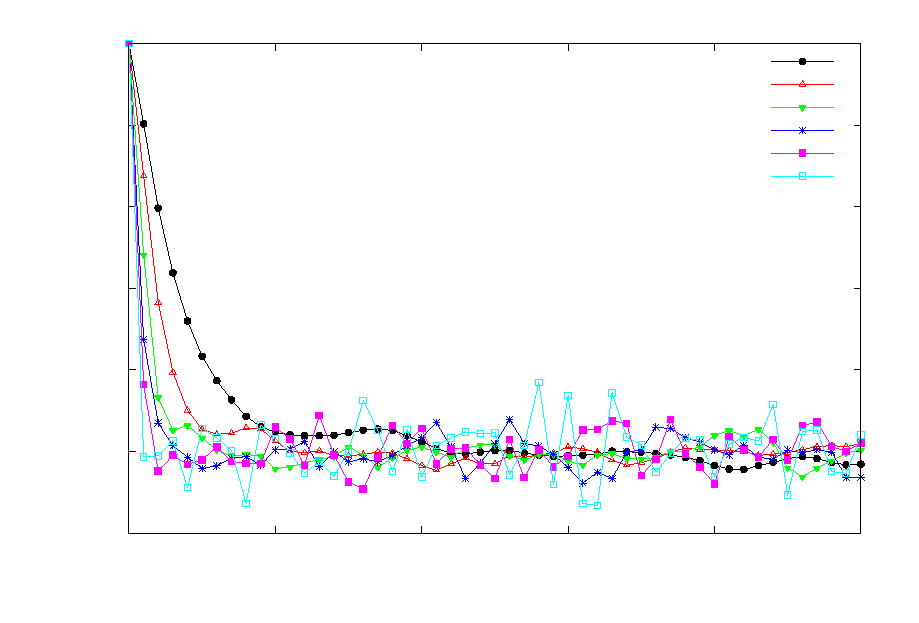
\includegraphics{correlationbinnmd100}}%
    \gplfronttext
  \end{picture}%
\endgroup

	\caption{Autocorrelation of the blocked Markov Chains for $N_{md}=100$}
	\label{fig:correlationbinnmd100}
\end{figure}

\subsection{Naive Standard errors of the blocked measurements}

\begin{figure}[htbp]
	% GNUPLOT: LaTeX picture with Postscript
\begingroup
  \makeatletter
  \providecommand\color[2][]{%
    \GenericError{(gnuplot) \space\space\space\@spaces}{%
      Package color not loaded in conjunction with
      terminal option `colourtext'%
    }{See the gnuplot documentation for explanation.%
    }{Either use 'blacktext' in gnuplot or load the package
      color.sty in LaTeX.}%
    \renewcommand\color[2][]{}%
  }%
  \providecommand\includegraphics[2][]{%
    \GenericError{(gnuplot) \space\space\space\@spaces}{%
      Package graphicx or graphics not loaded%
    }{See the gnuplot documentation for explanation.%
    }{The gnuplot epslatex terminal needs graphicx.sty or graphics.sty.}%
    \renewcommand\includegraphics[2][]{}%
  }%
  \providecommand\rotatebox[2]{#2}%
  \@ifundefined{ifGPcolor}{%
    \newif\ifGPcolor
    \GPcolortrue
  }{}%
  \@ifundefined{ifGPblacktext}{%
    \newif\ifGPblacktext
    \GPblacktextfalse
  }{}%
  % define a \g@addto@macro without @ in the name:
  \let\gplgaddtomacro\g@addto@macro
  % define empty templates for all commands taking text:
  \gdef\gplbacktext{}%
  \gdef\gplfronttext{}%
  \makeatother
  \ifGPblacktext
    % no textcolor at all
    \def\colorrgb#1{}%
    \def\colorgray#1{}%
  \else
    % gray or color?
    \ifGPcolor
      \def\colorrgb#1{\color[rgb]{#1}}%
      \def\colorgray#1{\color[gray]{#1}}%
      \expandafter\def\csname LTw\endcsname{\color{white}}%
      \expandafter\def\csname LTb\endcsname{\color{black}}%
      \expandafter\def\csname LTa\endcsname{\color{black}}%
      \expandafter\def\csname LT0\endcsname{\color[rgb]{1,0,0}}%
      \expandafter\def\csname LT1\endcsname{\color[rgb]{0,1,0}}%
      \expandafter\def\csname LT2\endcsname{\color[rgb]{0,0,1}}%
      \expandafter\def\csname LT3\endcsname{\color[rgb]{1,0,1}}%
      \expandafter\def\csname LT4\endcsname{\color[rgb]{0,1,1}}%
      \expandafter\def\csname LT5\endcsname{\color[rgb]{1,1,0}}%
      \expandafter\def\csname LT6\endcsname{\color[rgb]{0,0,0}}%
      \expandafter\def\csname LT7\endcsname{\color[rgb]{1,0.3,0}}%
      \expandafter\def\csname LT8\endcsname{\color[rgb]{0.5,0.5,0.5}}%
    \else
      % gray
      \def\colorrgb#1{\color{black}}%
      \def\colorgray#1{\color[gray]{#1}}%
      \expandafter\def\csname LTw\endcsname{\color{white}}%
      \expandafter\def\csname LTb\endcsname{\color{black}}%
      \expandafter\def\csname LTa\endcsname{\color{black}}%
      \expandafter\def\csname LT0\endcsname{\color{black}}%
      \expandafter\def\csname LT1\endcsname{\color{black}}%
      \expandafter\def\csname LT2\endcsname{\color{black}}%
      \expandafter\def\csname LT3\endcsname{\color{black}}%
      \expandafter\def\csname LT4\endcsname{\color{black}}%
      \expandafter\def\csname LT5\endcsname{\color{black}}%
      \expandafter\def\csname LT6\endcsname{\color{black}}%
      \expandafter\def\csname LT7\endcsname{\color{black}}%
      \expandafter\def\csname LT8\endcsname{\color{black}}%
    \fi
  \fi
    \setlength{\unitlength}{0.0500bp}%
    \ifx\gptboxheight\undefined%
      \newlength{\gptboxheight}%
      \newlength{\gptboxwidth}%
      \newsavebox{\gptboxtext}%
    \fi%
    \setlength{\fboxrule}{0.5pt}%
    \setlength{\fboxsep}{1pt}%
\begin{picture}(8502.00,5668.00)%
    \gplgaddtomacro\gplbacktext{%
      \csname LTb\endcsname%
      \put(1078,704){\makebox(0,0)[r]{\strut{}$0.001$}}%
      \put(1078,1487){\makebox(0,0)[r]{\strut{}$0.002$}}%
      \put(1078,2270){\makebox(0,0)[r]{\strut{}$0.003$}}%
      \put(1078,3054){\makebox(0,0)[r]{\strut{}$0.004$}}%
      \put(1078,3837){\makebox(0,0)[r]{\strut{}$0.005$}}%
      \put(1078,4620){\makebox(0,0)[r]{\strut{}$0.006$}}%
      \put(1078,5403){\makebox(0,0)[r]{\strut{}$0.007$}}%
      \put(1210,484){\makebox(0,0){\strut{}$2$}}%
      \put(2589,484){\makebox(0,0){\strut{}$4$}}%
      \put(3968,484){\makebox(0,0){\strut{}$8$}}%
      \put(5347,484){\makebox(0,0){\strut{}$16$}}%
      \put(6726,484){\makebox(0,0){\strut{}$32$}}%
      \put(8105,484){\makebox(0,0){\strut{}$64$}}%
    }%
    \gplgaddtomacro\gplfronttext{%
      \csname LTb\endcsname%
      \put(176,3053){\rotatebox{-270}{\makebox(0,0){\strut{}$\langle m\rangle$}}}%
      \put(4657,154){\makebox(0,0){\strut{}binlength}}%
      \csname LTb\endcsname%
      \put(2266,5230){\makebox(0,0)[r]{\strut{}$N_{md}=4$}}%
      \csname LTb\endcsname%
      \put(2266,5010){\makebox(0,0)[r]{\strut{}$N_{md}=100$}}%
    }%
    \gplbacktext
    \put(0,0){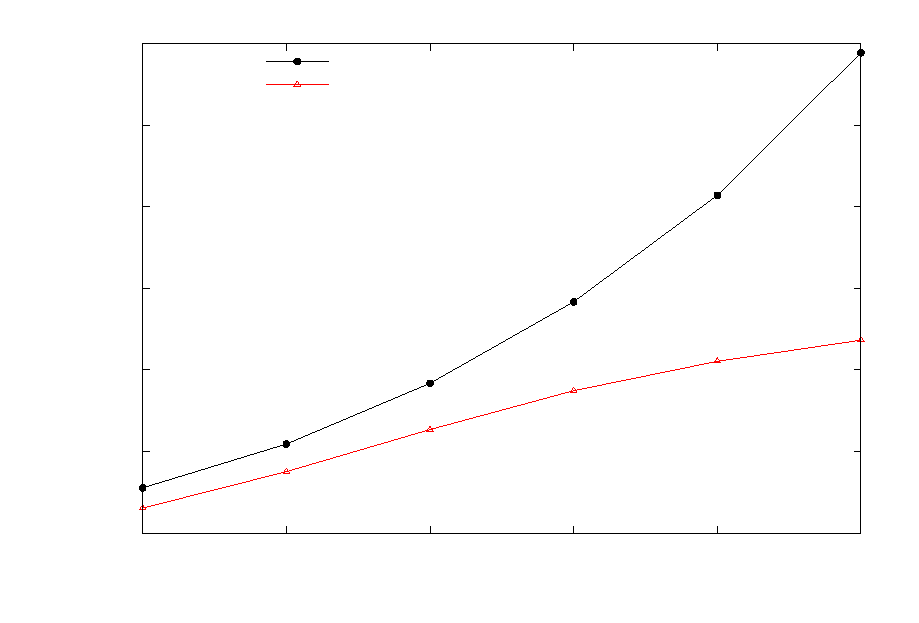
\includegraphics{naiveerrorbinned}}%
    \gplfronttext
  \end{picture}%
\endgroup

	\caption{Naive error of the blocked data}
	\label{fig:naiveerrorbinned}
\end{figure}

\subsection{Bootstraperrors of the blocked measurements}

\begin{figure}[htbp]
	% GNUPLOT: LaTeX picture with Postscript
\begingroup
  \makeatletter
  \providecommand\color[2][]{%
    \GenericError{(gnuplot) \space\space\space\@spaces}{%
      Package color not loaded in conjunction with
      terminal option `colourtext'%
    }{See the gnuplot documentation for explanation.%
    }{Either use 'blacktext' in gnuplot or load the package
      color.sty in LaTeX.}%
    \renewcommand\color[2][]{}%
  }%
  \providecommand\includegraphics[2][]{%
    \GenericError{(gnuplot) \space\space\space\@spaces}{%
      Package graphicx or graphics not loaded%
    }{See the gnuplot documentation for explanation.%
    }{The gnuplot epslatex terminal needs graphicx.sty or graphics.sty.}%
    \renewcommand\includegraphics[2][]{}%
  }%
  \providecommand\rotatebox[2]{#2}%
  \@ifundefined{ifGPcolor}{%
    \newif\ifGPcolor
    \GPcolortrue
  }{}%
  \@ifundefined{ifGPblacktext}{%
    \newif\ifGPblacktext
    \GPblacktextfalse
  }{}%
  % define a \g@addto@macro without @ in the name:
  \let\gplgaddtomacro\g@addto@macro
  % define empty templates for all commands taking text:
  \gdef\gplbacktext{}%
  \gdef\gplfronttext{}%
  \makeatother
  \ifGPblacktext
    % no textcolor at all
    \def\colorrgb#1{}%
    \def\colorgray#1{}%
  \else
    % gray or color?
    \ifGPcolor
      \def\colorrgb#1{\color[rgb]{#1}}%
      \def\colorgray#1{\color[gray]{#1}}%
      \expandafter\def\csname LTw\endcsname{\color{white}}%
      \expandafter\def\csname LTb\endcsname{\color{black}}%
      \expandafter\def\csname LTa\endcsname{\color{black}}%
      \expandafter\def\csname LT0\endcsname{\color[rgb]{1,0,0}}%
      \expandafter\def\csname LT1\endcsname{\color[rgb]{0,1,0}}%
      \expandafter\def\csname LT2\endcsname{\color[rgb]{0,0,1}}%
      \expandafter\def\csname LT3\endcsname{\color[rgb]{1,0,1}}%
      \expandafter\def\csname LT4\endcsname{\color[rgb]{0,1,1}}%
      \expandafter\def\csname LT5\endcsname{\color[rgb]{1,1,0}}%
      \expandafter\def\csname LT6\endcsname{\color[rgb]{0,0,0}}%
      \expandafter\def\csname LT7\endcsname{\color[rgb]{1,0.3,0}}%
      \expandafter\def\csname LT8\endcsname{\color[rgb]{0.5,0.5,0.5}}%
    \else
      % gray
      \def\colorrgb#1{\color{black}}%
      \def\colorgray#1{\color[gray]{#1}}%
      \expandafter\def\csname LTw\endcsname{\color{white}}%
      \expandafter\def\csname LTb\endcsname{\color{black}}%
      \expandafter\def\csname LTa\endcsname{\color{black}}%
      \expandafter\def\csname LT0\endcsname{\color{black}}%
      \expandafter\def\csname LT1\endcsname{\color{black}}%
      \expandafter\def\csname LT2\endcsname{\color{black}}%
      \expandafter\def\csname LT3\endcsname{\color{black}}%
      \expandafter\def\csname LT4\endcsname{\color{black}}%
      \expandafter\def\csname LT5\endcsname{\color{black}}%
      \expandafter\def\csname LT6\endcsname{\color{black}}%
      \expandafter\def\csname LT7\endcsname{\color{black}}%
      \expandafter\def\csname LT8\endcsname{\color{black}}%
    \fi
  \fi
    \setlength{\unitlength}{0.0500bp}%
    \ifx\gptboxheight\undefined%
      \newlength{\gptboxheight}%
      \newlength{\gptboxwidth}%
      \newsavebox{\gptboxtext}%
    \fi%
    \setlength{\fboxrule}{0.5pt}%
    \setlength{\fboxsep}{1pt}%
\begin{picture}(8502.00,5668.00)%
    \gplgaddtomacro\gplbacktext{%
      \csname LTb\endcsname%
      \put(1078,704){\makebox(0,0)[r]{\strut{}$0.001$}}%
      \put(1078,1487){\makebox(0,0)[r]{\strut{}$0.002$}}%
      \put(1078,2270){\makebox(0,0)[r]{\strut{}$0.003$}}%
      \put(1078,3054){\makebox(0,0)[r]{\strut{}$0.004$}}%
      \put(1078,3837){\makebox(0,0)[r]{\strut{}$0.005$}}%
      \put(1078,4620){\makebox(0,0)[r]{\strut{}$0.006$}}%
      \put(1078,5403){\makebox(0,0)[r]{\strut{}$0.007$}}%
      \put(1210,484){\makebox(0,0){\strut{}$2$}}%
      \put(2589,484){\makebox(0,0){\strut{}$4$}}%
      \put(3968,484){\makebox(0,0){\strut{}$8$}}%
      \put(5347,484){\makebox(0,0){\strut{}$16$}}%
      \put(6726,484){\makebox(0,0){\strut{}$32$}}%
      \put(8105,484){\makebox(0,0){\strut{}$64$}}%
    }%
    \gplgaddtomacro\gplfronttext{%
      \csname LTb\endcsname%
      \put(176,3053){\rotatebox{-270}{\makebox(0,0){\strut{}$\langle m\rangle$}}}%
      \put(4657,154){\makebox(0,0){\strut{}binlength}}%
      \csname LTb\endcsname%
      \put(2266,5230){\makebox(0,0)[r]{\strut{}$N_{md}=4$}}%
      \csname LTb\endcsname%
      \put(2266,5010){\makebox(0,0)[r]{\strut{}$N_{md}=100$}}%
    }%
    \gplbacktext
    \put(0,0){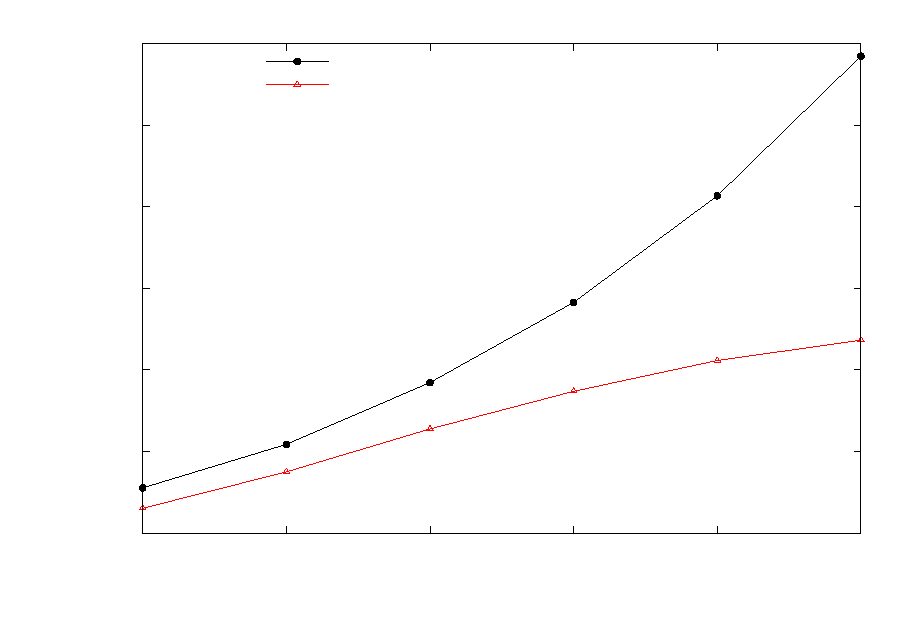
\includegraphics{bootstraperrorbinned}}%
    \gplfronttext
  \end{picture}%
\endgroup

	\caption{Bootsstrap error of the blocked data for $N_bs=4\cdot N$}
	\label{fig:bootstraperrorbinned}
\end{figure}

\begin{figure}[htbp]
	% GNUPLOT: LaTeX picture with Postscript
\begingroup
  \makeatletter
  \providecommand\color[2][]{%
    \GenericError{(gnuplot) \space\space\space\@spaces}{%
      Package color not loaded in conjunction with
      terminal option `colourtext'%
    }{See the gnuplot documentation for explanation.%
    }{Either use 'blacktext' in gnuplot or load the package
      color.sty in LaTeX.}%
    \renewcommand\color[2][]{}%
  }%
  \providecommand\includegraphics[2][]{%
    \GenericError{(gnuplot) \space\space\space\@spaces}{%
      Package graphicx or graphics not loaded%
    }{See the gnuplot documentation for explanation.%
    }{The gnuplot epslatex terminal needs graphicx.sty or graphics.sty.}%
    \renewcommand\includegraphics[2][]{}%
  }%
  \providecommand\rotatebox[2]{#2}%
  \@ifundefined{ifGPcolor}{%
    \newif\ifGPcolor
    \GPcolortrue
  }{}%
  \@ifundefined{ifGPblacktext}{%
    \newif\ifGPblacktext
    \GPblacktextfalse
  }{}%
  % define a \g@addto@macro without @ in the name:
  \let\gplgaddtomacro\g@addto@macro
  % define empty templates for all commands taking text:
  \gdef\gplbacktext{}%
  \gdef\gplfronttext{}%
  \makeatother
  \ifGPblacktext
    % no textcolor at all
    \def\colorrgb#1{}%
    \def\colorgray#1{}%
  \else
    % gray or color?
    \ifGPcolor
      \def\colorrgb#1{\color[rgb]{#1}}%
      \def\colorgray#1{\color[gray]{#1}}%
      \expandafter\def\csname LTw\endcsname{\color{white}}%
      \expandafter\def\csname LTb\endcsname{\color{black}}%
      \expandafter\def\csname LTa\endcsname{\color{black}}%
      \expandafter\def\csname LT0\endcsname{\color[rgb]{1,0,0}}%
      \expandafter\def\csname LT1\endcsname{\color[rgb]{0,1,0}}%
      \expandafter\def\csname LT2\endcsname{\color[rgb]{0,0,1}}%
      \expandafter\def\csname LT3\endcsname{\color[rgb]{1,0,1}}%
      \expandafter\def\csname LT4\endcsname{\color[rgb]{0,1,1}}%
      \expandafter\def\csname LT5\endcsname{\color[rgb]{1,1,0}}%
      \expandafter\def\csname LT6\endcsname{\color[rgb]{0,0,0}}%
      \expandafter\def\csname LT7\endcsname{\color[rgb]{1,0.3,0}}%
      \expandafter\def\csname LT8\endcsname{\color[rgb]{0.5,0.5,0.5}}%
    \else
      % gray
      \def\colorrgb#1{\color{black}}%
      \def\colorgray#1{\color[gray]{#1}}%
      \expandafter\def\csname LTw\endcsname{\color{white}}%
      \expandafter\def\csname LTb\endcsname{\color{black}}%
      \expandafter\def\csname LTa\endcsname{\color{black}}%
      \expandafter\def\csname LT0\endcsname{\color{black}}%
      \expandafter\def\csname LT1\endcsname{\color{black}}%
      \expandafter\def\csname LT2\endcsname{\color{black}}%
      \expandafter\def\csname LT3\endcsname{\color{black}}%
      \expandafter\def\csname LT4\endcsname{\color{black}}%
      \expandafter\def\csname LT5\endcsname{\color{black}}%
      \expandafter\def\csname LT6\endcsname{\color{black}}%
      \expandafter\def\csname LT7\endcsname{\color{black}}%
      \expandafter\def\csname LT8\endcsname{\color{black}}%
    \fi
  \fi
    \setlength{\unitlength}{0.0500bp}%
    \ifx\gptboxheight\undefined%
      \newlength{\gptboxheight}%
      \newlength{\gptboxwidth}%
      \newsavebox{\gptboxtext}%
    \fi%
    \setlength{\fboxrule}{0.5pt}%
    \setlength{\fboxsep}{1pt}%
\begin{picture}(8502.00,5668.00)%
    \gplgaddtomacro\gplbacktext{%
      \csname LTb\endcsname%
      \put(1210,704){\makebox(0,0)[r]{\strut{}$0.001$}}%
      \put(1210,1226){\makebox(0,0)[r]{\strut{}$0.0015$}}%
      \put(1210,1748){\makebox(0,0)[r]{\strut{}$0.002$}}%
      \put(1210,2270){\makebox(0,0)[r]{\strut{}$0.0025$}}%
      \put(1210,2792){\makebox(0,0)[r]{\strut{}$0.003$}}%
      \put(1210,3315){\makebox(0,0)[r]{\strut{}$0.0035$}}%
      \put(1210,3837){\makebox(0,0)[r]{\strut{}$0.004$}}%
      \put(1210,4359){\makebox(0,0)[r]{\strut{}$0.0045$}}%
      \put(1210,4881){\makebox(0,0)[r]{\strut{}$0.005$}}%
      \put(1210,5403){\makebox(0,0)[r]{\strut{}$0.0055$}}%
      \put(1342,484){\makebox(0,0){\strut{}$2$}}%
      \put(2244,484){\makebox(0,0){\strut{}$8$}}%
      \put(3145,484){\makebox(0,0){\strut{}$32$}}%
      \put(4047,484){\makebox(0,0){\strut{}$128$}}%
      \put(4949,484){\makebox(0,0){\strut{}$512$}}%
      \put(5851,484){\makebox(0,0){\strut{}$2048$}}%
      \put(6752,484){\makebox(0,0){\strut{}$8192$}}%
      \put(7654,484){\makebox(0,0){\strut{}$32768$}}%
    }%
    \gplgaddtomacro\gplfronttext{%
      \csname LTb\endcsname%
      \put(176,3053){\rotatebox{-270}{\makebox(0,0){\strut{}$\langle m\rangle$}}}%
      \put(4723,154){\makebox(0,0){\strut{}$N_{bs}$}}%
      \csname LTb\endcsname%
      \put(3058,5230){\makebox(0,0)[r]{\strut{}binlength=2}}%
      \csname LTb\endcsname%
      \put(3058,5010){\makebox(0,0)[r]{\strut{}binlength=4}}%
      \csname LTb\endcsname%
      \put(3058,4790){\makebox(0,0)[r]{\strut{}binlength=8}}%
      \csname LTb\endcsname%
      \put(3058,4570){\makebox(0,0)[r]{\strut{}binlength=16}}%
      \csname LTb\endcsname%
      \put(3058,4350){\makebox(0,0)[r]{\strut{}binlength=32}}%
      \csname LTb\endcsname%
      \put(3058,4130){\makebox(0,0)[r]{\strut{}binlength=64}}%
    }%
    \gplbacktext
    \put(0,0){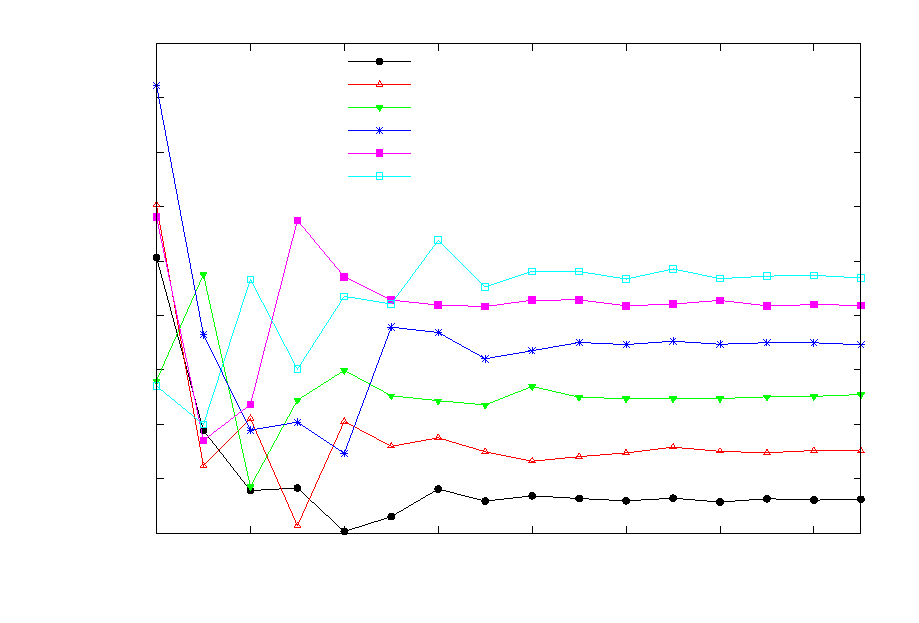
\includegraphics{errorstabilitynmd100}}%
    \gplfronttext
  \end{picture}%
\endgroup

	\caption{Stability of the bootstrap errors for different binlengths and $N_{bs}$, for $N_{md}=100$}
	\label{fig:errorstabilitynmd100}
\end{figure}
\newpage	
\listoffigures
\printbibliography
\end{document}